%!TEX root= ../../../report.tex

\section{Kinematic model}
\label{sec_kinematic_model}
The kinematics model of the robot describes the motion of every joint in time disregarding dynamic parameters.
It is used here to compute position, velocity and acceleration of the limbs for given trajectories of the toes, which are the contact point with the ground in the presented study case, through their forward kinematics.
Also the inverse kinematic model is constructed as a tool for the posterior computation of the dynamics model and its application to model the necessary actuators.
The model has been obtained through direct application of trigonometry instead of using the D-H parameters given its simplicity.
To do so, as explained before the case has been reduced to a two-dimensional study of one leg, where each robot leg has been analyzed as a kinematic chain of three degrees of freedom.
The main reference frame has been placed attached to the hip with its Y axis parallel to the ground, as if this was the base of a robotic arm, and the toe was the tool, has shown in Figure \ref{fig:kinematics}.
This representation has been chosen to ease the construction of the mathematical model.
\begin{figure}[ht]
	\centering
	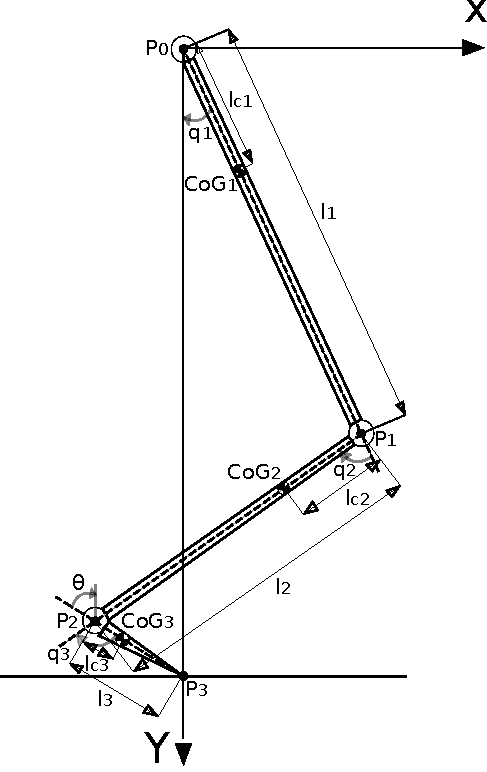
\includegraphics[width=0.4\textwidth]{figures/kinematics_model.pdf}
	\caption{Coordinate definitions for the schematic model of one leg}
	\label{fig:kinematics}
\end{figure}
The Figure \ref{fig:kinematics} depicts the schematic representation of only one leg, since the other one is equivalent. 
The system is said to be in single support phase since there would be just one foot in contact to the ground.
In the analyzed case, the swinging leg (not represented in Figure \ref{fig:kinematics}) would be static and could be considered an additional link with no degrees of freedom.
The variables $q_{i}$ represent the angles of the joints with respect to their fully-stretched positions to simplify the obtainment of the forward kinematic model, while the angle $\Theta$ is used to express the orientation of the ankle in an absolute manner. 
From Figure \ref{fig:kinematics}, the forward kinematic model in \ref{eq:forward_kinematics} can be easily obtained.
\begin{equation}
\label{eq:forward_kinematics}
	\begin{aligned}
		x_{0} &= 0 \\
		y_{0} &= 0 \\
		x_{1} &= l_{1} \sin(q_{1}) \\
		y_{1} &= l_{1} \cos(q_{1}) \\
		x_{2} &= l_{1} \sin(q_{1}) + l_{2} \sin(q_{1}+q_{2}) \\
		y_{2} &= l_{1} \cos(q_{1}) + l_{2} \cos(q_{1}+q_{2}) \\
		x_{3} &= l_{1} \sin(q_{1}) + l_{2} \sin(q_{1}+q_{2}) + l_{3} \sin(q_{1}+q_{2}+q_{3}) \\
		y_{3} &= l_{1} \cos(q_{1}) + l_{2} \cos(q_{1}+q_{2}) + l_{3} \cos(q_{1}+q_{2}+q_{3}) 
	\end{aligned}
\end{equation}
The variables $x_{i}, y_{i}$ represent the position coordinates of the joints in the right leg, named $P_{i}$ in the schematic in Figure \ref{fig:kinematics} and $P'_{i}$ for the left leg (not depicted).
Once computed, the linear velocity and acceleration of every joint can be obtained by derivation of the forward kinematic model and represented as $\dot{P}_{i}$ and $\ddot{P}_{i}$.

The model presented is the most basic one and does not contain the degrees of freedom that could be introduced by springs in the actuators.
This is due to two reasons:
\begin{itemize}
	\item Their configuration can be changed to series, parallel or none in both knees and ankles.
	\item The study of the jump case regarding the parameterization of the actuators has been carried out in the most disadvantageous scenario from the energetic point of view, which in this case means no springs.
\end{itemize}

Following the same approach, the inverse kinematic model can be computed for the right leg, yielding the equations \ref{eq:inverse_kinematics}.
\begin{equation}
\label{eq:inverse_kinematics}
	\begin{aligned}
		x_{2} &= x_{3} - l_{3} \sin(\Theta) \\
		y_{2} &= y_{3} - l_{3} \cos(\Theta) \\
		q_{1} &= \arctan \left(\frac{x_{2}}{y_{2}}\right) - \arccos \left(\frac{x_{2}^2 + y_{2}^2 + l_{1}^2 - l_{2}^2}{2 l_{1} \sqrt{x_{2}^2 + y_{2}^2}}\right) \\
		q_{2} &= \pi - \arccos \left(\frac{l_{1}^2 + l_{2}^2 - x_{2} - y_{2}}{2 l_{1} l_{2}}\right) \\
		q_{3} &= \Theta - q_{1} - q_{2} \\
	\end{aligned}
\end{equation}
And equivalently to the forward kinematics, the inverse kinematic model can be derived to obtain the velocities and accelerations in the joint space $\dot{q_{i}}$ and $\ddot{q_{i}}$.
